\documentclass{article}

% if you need to pass options to natbib, use, e.g.:
% \PassOptionsToPackage{numbers, compress}{natbib}
% before loading nips_2016
%
% to avoid loading the natbib package, add option nonatbib:
% \usepackage[nonatbib]{nips_2016}

% \usepackage{nips_2016}

% to compile a camera-ready version, add the [final] option, e.g.:

\PassOptionsToPackage{square,numbers}{natbib}

\usepackage[final]{nips_2016}

\usepackage[utf8]{inputenc} % allow utf-8 input
\usepackage[T1]{fontenc}    % use 8-bit T1 fonts
\usepackage{hyperref}       % hyperlinks
\usepackage{url}            % simple URL typesetting
\usepackage{booktabs}       % professional-quality tables
\usepackage{amsfonts}       % blackboard math symbols
\usepackage{nicefrac}       % compact symbols for 1/2, etc.
\usepackage{microtype}      % microtypography
\usepackage{amsmath}
\usepackage{graphicx}
\graphicspath{ {images/} }
\usepackage{subfig}
\usepackage{multirow}
\usepackage{algorithm}
\usepackage[utf8]{inputenc} % allow utf-8 input
\usepackage[T1]{fontenc}    % use 8-bit T1 fonts
\usepackage{hyperref}       % hyperlinks
\usepackage{url}            % simple URL typesetting
\usepackage{booktabs}       % professional-quality tables
\usepackage{amsfonts}       % blackboard math symbols
\usepackage{nicefrac}       % compact symbols for 1/2, etc.
\usepackage{microtype}      % microtypography
\usepackage{amsmath}
\usepackage{graphicx}
\usepackage{media9} 
\usepackage{caption}
% \usepackage{subcaption}
\usepackage{amsmath}
\usepackage{algorithm, algpseudocode}
\usepackage{verbatim}

% \renewcommand{\baselinestretch}{0.90}

\usepackage{float}

\title{Zero Shot Learning of Vectorized Sketch Images}

\author{
  Nitish Kulkarni \\
  Carnegie Mellon University\\
  \texttt{nitishkk@cs.cmu.edu} \\
  \And
  Aditya Siddhant \\
  Carnegie Mellon University\\
  \texttt{asiddhan@cs.cmu.edu} \\
  \And
  George Tan \\
  Carnegie Mellon University\\
  \texttt{georget1@cs.cmu.edu} \\
}

\begin{document}
% \nipsfinalcopy is no longer used

\maketitle


\begin{abstract}
Use of neural networks for image generation has gained popularity in recent times.  Most of the work in this area has targeted the modeling of pixel images. However, humans do not learn to draw images as a matrix of pixels. They learn to represent the abstract concepts present in an object by using a sequence of strokes. We are therefore addressing the challenge of generating images, or rather sketches, in a vectorized manner given a pixel image of the object. Our goal is to train a generative model that learns to draw and generalize abstract concepts in a manner indistinguishable from humans. We also introduce dynamic time warping for quantitative evaluation of the model's sketches. We consider this problem as \textit{Zero Shot} because the problem entails generation different sketch representations of previously unseen objects in pixel images during test time.
\end{abstract}


\section{Introduction}

Handwriting synthesis and hand-drawn sketch generation have been recently successful with deep neural networks. These deep neural networks include recurrent neural networks (RNN) with Long Short-term Memory (LSTM) \cite{LSTM}, Generative Adversarial Networks (GAN) \cite{GAN}, and Variational Autoencoders (VAE) \cite{journals/corr/KingmaW13} which have all been demonstrated to generate human-level handwriting and sketches. However, these methods have not been utilized to generate sketches in a vectorized manner given a pixel image. This task is challenging since given an image, the sequential vector representation of the image is not immediately apparent. Our goal is to train the network to learn the high-level visual features of the pixel image and output sketch images that are represented as a sequence of pen stroke vectors in an end to end manner.

The goal stated above is naturally analogous to image captioning which is the problem generating natural sentences to describe a given image. Recent advances in image captioning lead to a generative model based on a deep recurrent neural network that combines advances in computer vision and machine translation. The model is the Neural Image Caption (NIC) \cite{DBLP:journals/corr/VinyalsTBE14} which is an end-to-end neural network with a Convolutional Neural Network (CNN) \cite{MNIST} for image feature learning followed by a language generating RNN that uses the image features from the CNN. 

In our problem of hand-drawn sketch generation given a pixel image, the sketch generation of a sequence of stroke vectors is analogous to the language generation of a sequence of words. We propose to borrow the ideas of the NIC model to create a deep neural network model to generate vectorized sketches represented as a sequence of strokes, given a pixel image. We evaluate the vectorized sketches with dynamic time warping to measure the similarity between the two temporal sequences since the strokes may vary in size and length.


\section{Related Work}

Recurrent Neural Networks models have been used as generative models for modeling different type of sequences. RNNs with LSTM were used for handwriting synthesis i.e. generate handwritten characters for a given text \cite{DBLP:journals/corr/Graves13} which are times series data. GANs, a framework to estimate generative models with an adversarial process, have been demonstrated to generate images of hand-written digits from MNIST \cite{MNIST}, faces from the Toronto Face Database \cite{TFD}, and various objects from CIFAR \cite{CIFAR} when given an image of some arbitrary noise. VAEs, a generative model with an encoder and decoder architecture, can generate street view house numbers \cite{DBLP:journals/corr/GregorDGW15} and sketch images \cite{qdpaper} by sampling the latent variable from a unit Gaussian distribution. Another sequence generation task that has received a lot of attention is the image captioning task. Recent improvements in image captioning include Show and Tell \cite{DBLP:journals/corr/VinyalsTBE14} and a Multimodal Recurrent Neural Network \cite{DBLP:journals/corr/KarpathyF14} that uses an architecture that is a CNN followed by a language generating RNN.

Although freehand sketches have not received as much attention as pixel images, there has some work in recognition of freehand sketches using deep neural networks. Some works have tried to complete the sketch conditioned on first few strokes and try to build a system for guiding the free-form drawing of objects \cite{qdpaper} \cite{rcp2}. Other works have tried to retrieve the pixel image of an object given the sketch \cite{sketchydb} where one uses the deep features of the sketches \cite{rcp1}. One work has shown to mimic and recreate similar looking drawings from given drawings with generative models \cite{qdpaper}. To the best of our knowledge, there is no work that has used a multimodal deep learning approach to generate vectorized sketches using a pixel image.

In previous image captioning works, images are captioned by separating the image into sub-images and mapping the sub-images to word terms \cite{Hironobu99}. The sub-images to word terms mapping were also learned by an EM algorithm \cite{Duygulu2002}. Recent improvements in image captioning include Show and Tell \cite{DBLP:journals/corr/VinyalsTBE14} and a Multimodal Recurrent Neural Network \cite{DBLP:journals/corr/KarpathyF14} that uses an architecture that is a CNN followed by a language generating RNN.


\section{Dataset}

One of the significant challenges faced in this work is that there is no publicly available source of substantial data that comprises pixel image - vector image pairs required to learn a generative model we describe. However, there are many sources that consist of large collections of text-annotated data for pixel images and vector images individually. We leverage the availability of these datasets to curate our dataset by associating the pixel images to the vector images using an ensemble of similarity techniques.

As a primary source of vector images, we use the Quick Draw dataset \cite{quickdraw}. The dataset consists of over 50 million drawings of 200 objects contributed by over 15 million players who played Google’s drawing game, "Quick, Draw!". The dataset also contains the players' strokes and the sequence of the strokes to create each drawing, which is essential for the CNN-Sketch-RNN model. In the context of this work, we use 50 categories with 1000 sketches each for training and 50 categories with 1000 sketches each for testing. We manually collected pixel images from multiple sources on the web corresponding to the categories in Quick Draw Dataset.

\begin{figure}[H]
\centering
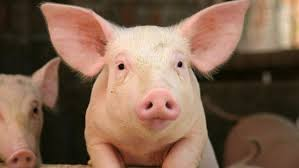
\includegraphics[width=1.5cm]{images/pig.jpg}
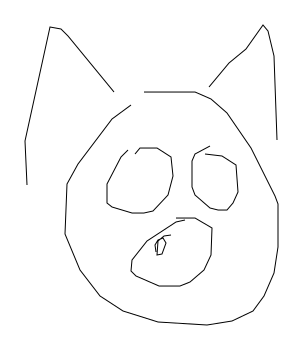
\includegraphics[width=1.5cm]{images/pig00008.png}
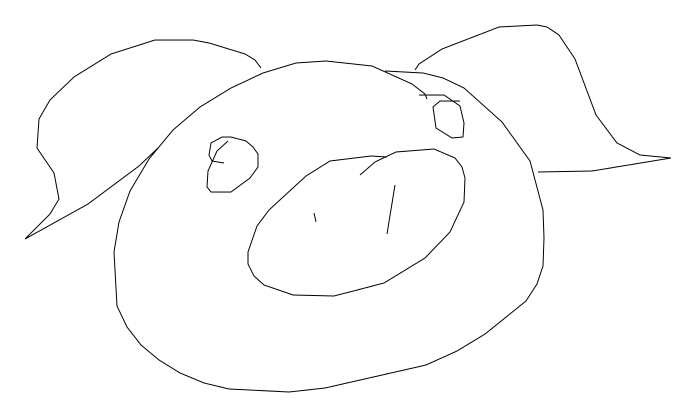
\includegraphics[width=1.5cm]{images/pig00039.png}
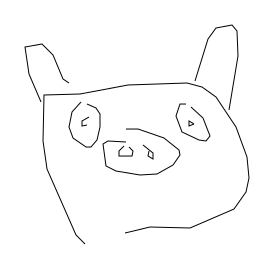
\includegraphics[width=1.5cm]{images/pig00161.png}
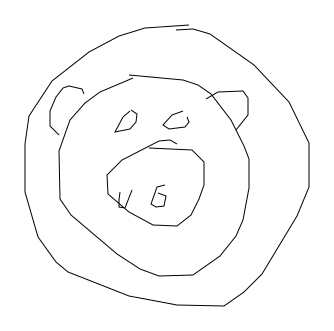
\includegraphics[width=1.5cm]{images/pig00295.png}\\
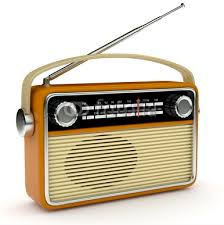
\includegraphics[width=1.5cm]{images/radio.jpg}
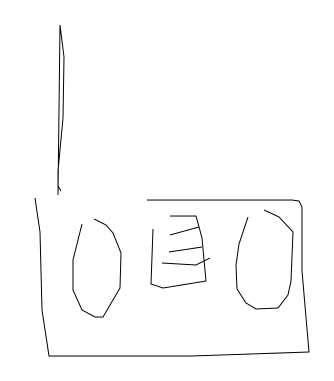
\includegraphics[width=1.5cm]{images/radio00008.png}
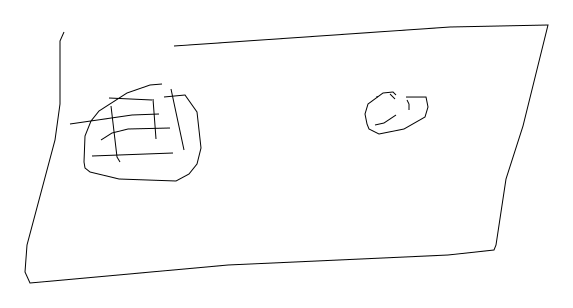
\includegraphics[width=1.5cm]{images/radio00111.png}
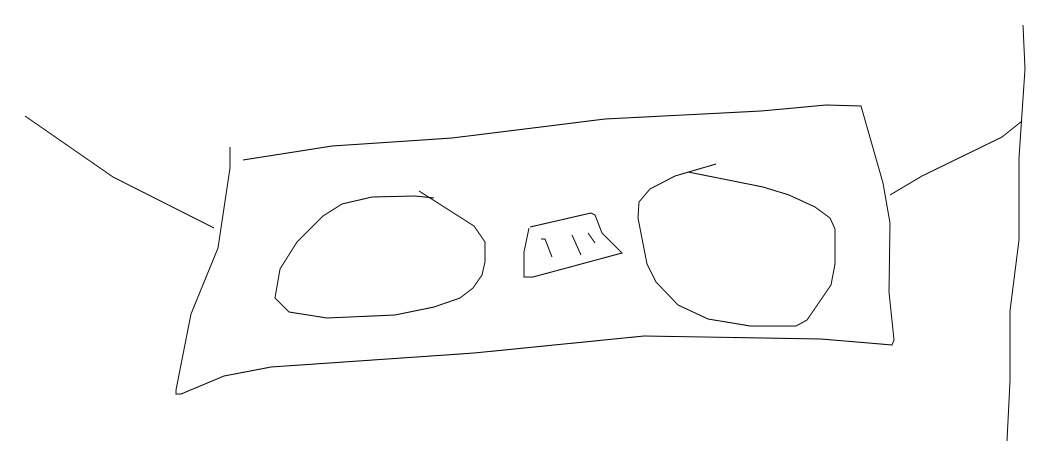
\includegraphics[width=1.5cm]{images/radio00161.png}
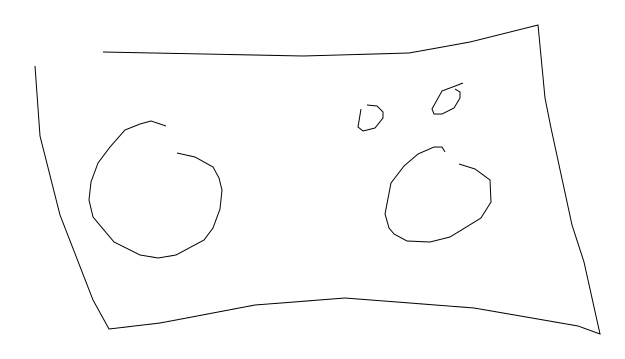
\includegraphics[width=1.5cm]{images/radio00286.png}\\
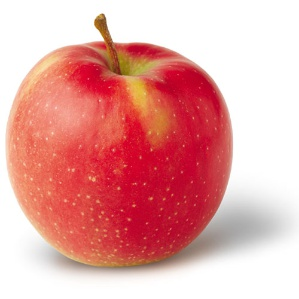
\includegraphics[width=1.5cm]{images/apple01.jpg}
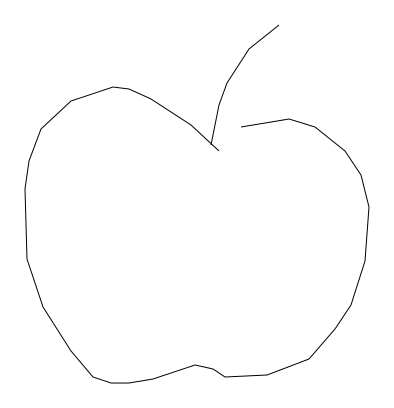
\includegraphics[width=1.5cm]{images/apple00247(1).png}
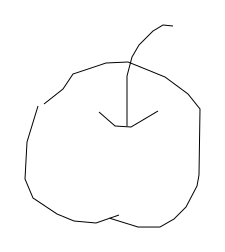
\includegraphics[width=1.5cm]{images/apple00247(2).png}
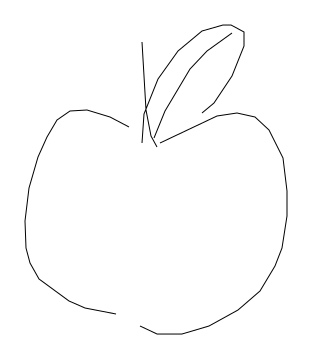
\includegraphics[width=1.5cm]{images/apple00247(3).png}
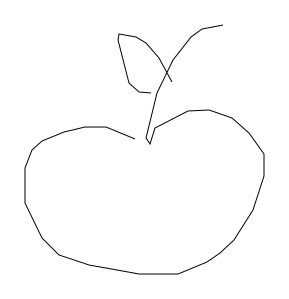
\includegraphics[width=1.5cm]{images/apple00247(4).png}\\
\caption{Pixel images of a  collected from the web and their four sketches selected from the Quick Draw dataset \cite{quickdraw}}
\end{figure}

Having collected the vector and pixel images for different categories, we generate image-sketch pairs in order to train the CNN-Sketch-RNN model. For training the model, we have considered 60 image categories, with 1000 vector images. Since most of the final sketches were highly similar, to pair the images with the sketches, we used k-means clustering  (with $k = 5$) to cluster the sketches, and we manually associated each cluster to the pixel image that is most visually similar to the cluster mean. We clustered over the pixel coordinates and chose the fixed number of clusters based on the most common number of clusters.

\subsection{Data Pre-processing}
The input to the network is the pixel image represented as a matrix where $I$ is the pixel image and $I\in \mathbb{R}^{m\times n\times c}$ so the input image pixel has a height of $m$ and width of $n$ and $c$ channels. The output of the network represents a sketch as a set of pen stroke actions as used by sketch-rnn \cite{qdpaper}. A single stroke action vector consists of five elements $(\Delta x, \Delta y, p_{1}, p_{2}, p_{3})$ where $\Delta x, \Delta y$ are the pen's offsets in the x and y direction to the next state and $p_{1}, p_{2}, p_{3}$ are the pen's state where $p_{1}$ indicates that the pen is touching the paper, $p_{2}$ indicates that the pen is lifted from the paper, and $p_{3}$ indicates that the drawing is over. Given a sequence of the stroke action vectors $s = (s_{0}, ..., s_{N-1})$, a sketch image can be constructed as describe by sketch-rnn \cite{qdpaper}.


\section{Method}

To learn a generative model for vector images, we explore an extension of the multimodal NIC model from Show and Tell \cite{DBLP:journals/corr/VinyalsTBE14} which is an end-to-end neural network with CNN for feature learning on the image followed by a language generating RNN that uses the features from the CNN. Analogous to image captioning, regions of the image can be mapped to pen strokes where a sequence of those pen strokes would construct the sketch of the input pixel image. We use the CNN learn the encoding of pixel image into the latent variable and the LSTM RNN decodes the latent variable into a sequence of strokes. A correct sketch can be defined by the correctness of the stroke action vectors. Hence we propose to maximize the similarity of a generated stroke to target stroke.

In other words, we use the CNN in order to learn visual features and use the LSTM RNN to generate the pen strokes of the sketch image from the visual features. In order to learn the sequence of strokes in a sketch to imitate human-like behavior, we use RNNs. Since Long Short-Term Memory (LSTM) \cite{LSTM} memory cells are well-suited to learn and predict time series data. an RNN can be used generate the strokes of an object's sketch. The LSTM keeps a hidden state which learns the dependencies of the time series data. We plan to feed the encoding of pixel image into this RNN so that the stroke generation is conditioned on the pixel image.

\begin{comment}

\subsection{Formulation}
\begin{gather}
\hat{\theta} = arg\max_{\theta} \sum_{(I,s)} p(s|I;\theta)\\
p(s|I;\theta) = \sum_{t=0}^{N-1} p(s_{t}|I,s_{t-1}, ..., s_{0};\theta)
\end{gather}

The formulation for the problem is described in the equations above where $I$ is the input image, $s$ is the sequence of strokes $s_{0}, ..., s_{N-1}$ to generate the sketch image that corresponds to $I$, and $\theta$ are the parameters of the model. Since $s$ is a sequence of strokes, then the joint probability of $s$ is dependent on individual strokes $s_{0}, ..., s_{N-1}$ where the strokes are dependent on previous strokes i.e. $s_{t}$ is dependent on $s_{t-1}, ..., s_{0}$. It would be natural to model $p(s_{t}|I,s_{t-1}, ..., s_{0};\theta)$ with an RNN where $I$ is processed with a CNN.

\end{comment}

\subsection{CNN RNN Model}
\begin{figure}[h]
\centering
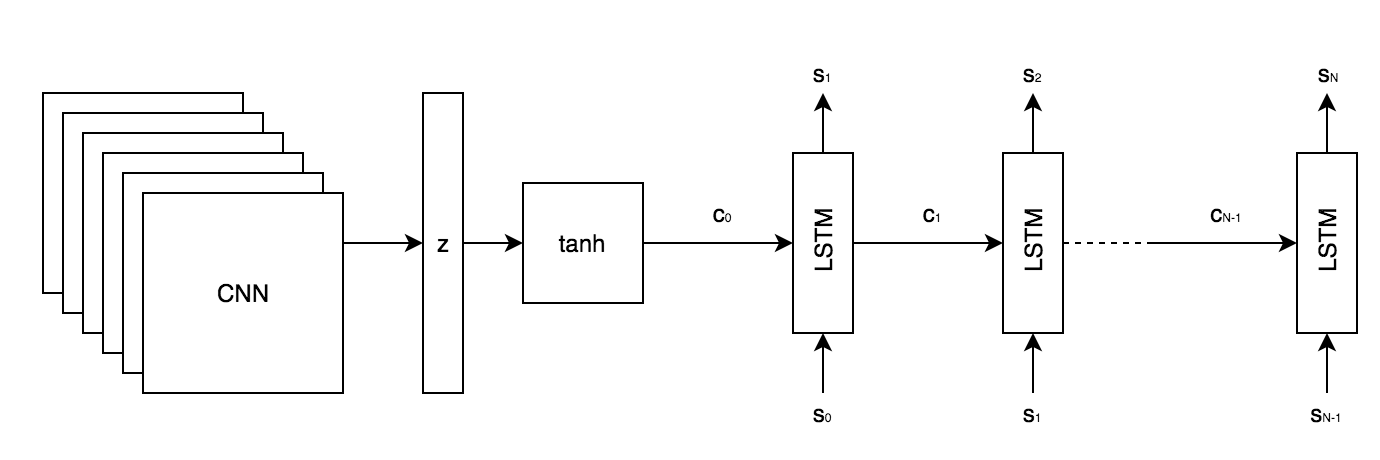
\includegraphics[width=12cm]{images/midterm_model.png}
\caption{CNN RNN Model Architechture}
\end{figure}

Let $I$ denote the input pixel image and $s = (s_{0}, ..., s_{N-1})$ be the vector sequence that constructs the sketch image where $s_{t} = (\Delta x_{t}, \Delta y_{t}, p_{t, 1}, p_{t, 2}, p_{t, 3})$ at some time step $t$. The pixel image $I$ would be the input to the deep CNN for visual feature extraction. Using the output of the CNN, the LSTM RNN would output the vector sequence $s_{0}, ..., s_{N-1}$. The forward procedure is

\begin{align*}
z &= CNN(I), c_{0} = tanh(z), h_{0} = 0\\
[h_{t+1}; c_{t+1}] &= LSTM([z;\hat{s}_{t}], [h_{t}; c_{t}])\\
y_{t+1} &= Linear(h_{t+1}), y_{t+1}\in\mathbb{R}^{5}\\
\hat{s}_{t+1} &= (y_{t+1,1}, y_{t+1,2}, softmax(y_{t+1,3}, y_{t+1,4}, y_{t+1,5}))
\end{align*}

for $t\in \{0, ..., N-1\}$ where z is the latent vector which is the output of the CNN "encoder" and the concatenated vector of z and $\hat{s}_{t}$ is fed into the LSTM "decoder" to generate the next pen stroke action $\hat{s}_{t+1}$ starting at $\hat{s}_{0} = (0,0,1,0,0)$. For the ground-truth sketch sequence $s = (s_{0}, ..., s_{N-1})$ and predicted output sketch sequence $\hat{s} = (\hat{s}_{0}, ..., \hat{s}_{N-1})$, the loss is defined as

\begin{align*}
L_{total}(s, \hat{s}) &= L_{C}(s, \hat{s}) + L_{CE}(s, \hat{s})\\
L_{C}(s, \hat{s}) &= \sum_{t=0}^{N-1} (\Delta x_{t} - \Delta \hat{x}_{t})^{2} + (\Delta y_{t} - \Delta \hat{y}_{t})^{2}\\
L_{CE}(s, \hat{s}) &= \sum_{t=0}^{N-1} \sum_{i=0}^{2} p_{t,i} log(\hat{p}_{t,i})
\end{align*}

where $L_{C}$ is the construction loss i.e. the L2 loss of the offsets, $L_{CE}$ is the cross-entropy loss of the pen's categorical state, and $L_{total}$ is the total loss which sums up the L2 loss of the offsets and the cross-entropy loss of the pen's state.


\subsection{CNN Sketch RNN Model}
Directly learning the pen's offset $(\Delta x, \Delta y)$ is not as generalized. Instead, we learn the distribution of the offsets $(\Delta x, \Delta y)$ instead of having a deterministic output. The offsets $(\Delta x, \Delta y)$ could be modelled as a Gaussian Mixture Model (GMM) with M bivariate normal distributions \cite{DBLP:journals/corr/Graves13}. Hence instead of $(\Delta x, \Delta y)$ as the output from the LSTM, the output is $(\pi, \mu_{x}, \mu_{y}, \sigma_{x}, \sigma_{y}, \rho_{xy})$ at each time step where $p(\Delta x, \Delta y) = \sum_{i=1}^{M} \pi_{i} \mathcal{N}(\Delta x_{i}, \Delta y_{i} | \mu_{x, i}, \mu_{y, i}, \sigma_{x, i}, \sigma_{y, i}, \rho_{xy, i})$ \cite{DBLP:journals/corr/Graves13}. Hence the offset is sampled from the GMM i.e. $\Delta x, \Delta y \sim GMM(\pi, \mu_{x}, \mu_{y}, \sigma_{x}, \sigma_{y}, \rho_{xy})$ instead of being directly computed by the model. This would allow a higher generalization of the pen strokes because the network learns the offset's distribution so we can sample the offset from the distribution instead.

\begin{figure}[h]
\centering
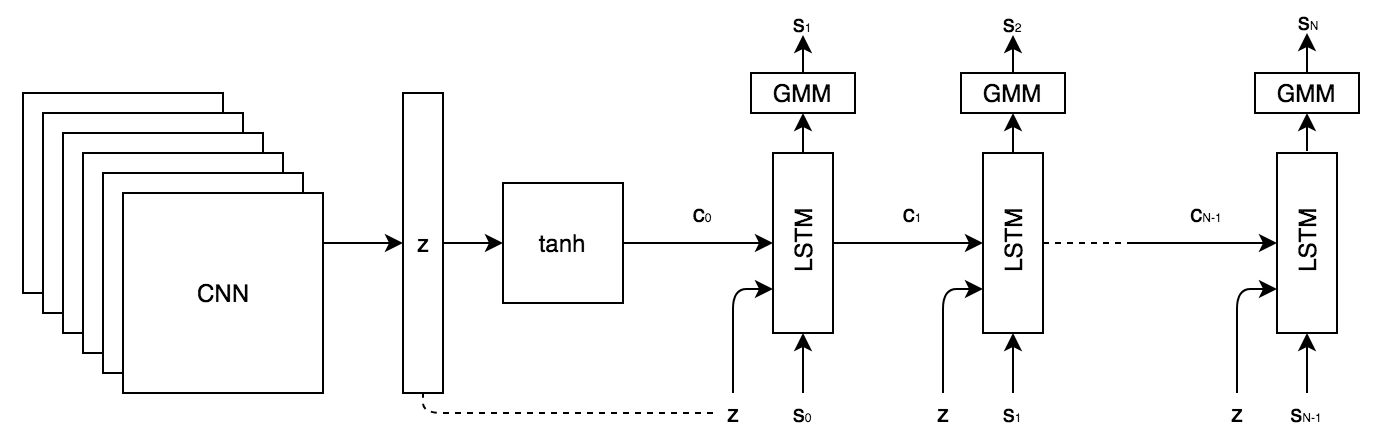
\includegraphics[width=12cm]{images/final_model.png}
\begin{comment}
The model was created on https://www.draw.io and the model.xml file in the folder is the XML of the model diagram.
\end{comment}
\caption{CNN Sketch RNN Model Architechture)}
\end{figure}

The equations would now be:

\begin{align*}
z &= CNN(I); c_{0} = tanh(z); h_{0} = 0\\
[h_{t+1}; c_{t+1}] &= LSTM([z; s_{t}], [h_{t}; c_{t}])\\
y_{t+1} &= Linear(h_{t+1}), y_{t+1}\in\mathbb{R}^{6M+3}\\
\Delta x, \Delta y &\sim GMM(y_{t+1, 0}, ..., y_{t+1, 6M-1})\\
p_{1}, p_{2}, p_{3} &= softmax(y_{t+1, 6M}, y_{t+1, 6M+1}, y_{t+1, 6M+2})\\
\hat{s}_{t+1} &= (\Delta x, \Delta y, p_{1}, p_{2}, p_{3})
\end{align*}

The Loss functions we have would now become:

\begin{align*}
L_{total}(s, \hat{s}) &= L_{C}(s, \hat{s}) + L_{CE}(s, \hat{s})\\
L_{C}(s, \hat{s}) &= -\frac{1}{N_{max}} \sum_{i=1}^{N_{s}} log(\sum_{j=1}^{M} \pi_{j,i} \mathcal{N}(\Delta x_{j, i}, \Delta y_{j, i} | \mu_{x, j, i}, \mu_{y, j, i}, \sigma_{x, j, i}, \sigma_{y, j, i}, \rho_{xy, j, i}))\\
L_{CE}(s, \hat{s}) &= \frac{1}{N_{max}} \sum_{t=0}^{N_{max}} \sum_{i=0}^{2} p_{i,t} log(\hat{p}_{i,t})
\end{align*}

where $L_{C}$ is the sum of the negative log-likelihoods of the offset distribution, $L_{CE}$ is the cross-entropy loss of the pen's categorical state, and $L_{total}$ is the total reconstruction loss which sums up the negative log-likelihoods and the cross-entropy loss of the pen's state \cite{qdpaper}.

\subsection{Evaluation} \label{sec:eval}

We consider multiple aspects of the model in order to fairly evaluate it, both qualitatively and quantitatively. For qualitative evaluation, we compare the strokes manually to the human-generated stokes for each category of images, and analyze the model behavior for different classes, which is explicated in greater detail in section \ref{sec:results}.

One of the biggest challenges of a generative model is the quantitative evaluation. A primary objective of the model is to draw strokes as close to humans as possible. We evaluate this ``closeness" from multiple viewpoints. For any image category, a test set of vector images is set aside for testing, which is considered as reference for evaluating the generated vector images for that category. 

As a first order similarity, we compare the final pixel image of the sketch to the pixel image of the human-drawn sketches. To compute the similarity, we first train a single hidden layer MLP to classify a sketch image into one of the 60 categories. As an evaluation metric for the similarity, we compute the prediction accuracy as well as compute cosine similarity of the hidden layer activations.

We also correlate the number of strokes generated by the CNN-Sketch-RNN model to the number of strokes used by humans as a second order similarity of the vector images. This is implemented as a cosine similarity of the normalized frequency vectors for a given image category as a cosine similarity of number of strokes (CosineSimCS) score i.e. 

\begin{align*}
    CosineSimCS(i, j) &= \mathbf{f}_i^T \mathbf{f}_j \\
    \text{where } \mathbf{f}_i[k] &= \text{fraction of images with $k$ strokes} \\
    MeanCosineSimCS(i) &= mean_{j \in Ref Sketches} CosineSimCS(i, j)
\end{align*}

As a third order similarity, we compute the temporal similarity of the individual strokes generated by the model with the human-drawn strokes. To do this, we use mean Dynamic Time Warping (DTW) distance as a metric for time-series similarity of the stroke-pixels. DTW gives a distance measure for two temporal sequences that may vary in speed and length. Since there can be multiple orderings and styles of strokes, we consider the minimum mean DTW distance among all the human-drawn sketches as the DTW score for a generated image. But this score tends to be biased towards categories that are less ambiguous and have low variance. To mitigate that, we fit a normal distribution over the DTW scores for the human-drawn images of a given category and use the $cdf$ of the DTW score of the generated vector image over this distribution as a category-wise Normalized DTW (NDTW) score.

\begin{align*}
    Mean\text{ }DTW\text{ }Dist(i, j) &= DTW\text{ }Distance(i, j) / Stroke\text{ }Length \\
    DTW\text{ }Score(i) &= min_{j \in refSketches} Mean\text{ }DTW\text{ }Dist(i, j) \\
    NDTW\text{ }Score(i) &= \mathcal{P}[ X > DTW\text{ }Score(i)] \\
    \text{where, }
    X &\sim \mathcal{N(\mu, \sigma)} \\
    \mu &= mean_{i \in refSketches}DTW\text{ }Score(i) \\
    \sigma &= std_{i \in refSketches}DTW\text{ }Score(i)
\end{align*}

With this formulation, the normalized DTW Score indicates the probability that the model-generated vector image mimics the reference sketches better than a random human-generated vector image (not in the reference sketches) for the same category.

For evaluating the zero-shot learning capabilities of the model, we generate vector images for image categories that were not included in the training set, and compute the same evaluation metrics discussed above for these vector images.

\section{Experiments and Results} \label{sec:results}

We trained the CNN-Sketch-RNN model to minimize the loss using the Adam Optimizer with learning rate 0.001 for 100 epochs with batch-size of 500. The CNN was the pre-trained 16-layer network used by the Visual Geometry Group (VGG) team \cite{VGG} where the weights are held constant with one fully connected layer from 4096 hidden units to 128 hidden units. The LSTM has hidden units 128 and back-propagation through time was done up to 250 time-steps.

We also run the model on our test images and images that the model has not seen before to generate the corresponding sketch image. Figure \ref{fig:sketches} shows the sketches of test images and images that the model has not seen before.

After training the model, we generate 100 vector images for each image category and compute the evaluation metrics discussed in section \ref{sec:eval}. The quantitative results for the generated images are tabulated in Table \ref{table:results_model1}. We report both overall and per-category metrics, where overall measure corresponds to the mean score for all the test instances and per-category score refers to mean of the individual category-wise means of scores.

\begin{table}[H]
    \centering
    \begin{tabular}{c|c|c|c} \toprule
        Metric & Human Drawn & CNN-RNN & CNN-Sketch-RNN \\ 
         & Sketches & Model Generated & Model Generated \\ 
         &  & Sketches & Sketches \\
         \hline
        MeanCosineSimCS (Overall) & - & 0.19  & 0.20 \\ \hline
        MeanCosineSimCS (Per-Category) & - & 0.18  & 0.21 \\ \hline
        NDTW score (Overall) & 0.51 & 0.12  & 0.11 \\ \hline
        NDTW score (Per-Category) &  0.52 & 0.16 & 0.14 \\ \hline
    \end{tabular}

    \caption{Evaluation metrics for Model 1: CNN RNN model}
    \label{table:results_model1}
\end{table}{}

% \begin{table}[H]
%     \centering
%     \begin{tabular}{c|c|c} \toprule
%         Metric & Human Drawn & CNN-Sketch-RNN \\ 
%          & Sketches & Model Generated  \\
%          &  & Sketches \\
%          \hline
%         Avg cosine similarity (Num strokes) (Overall) & - & 0.20  \\ \hline
%         Avg cosine similarity (Num strokes) (Per-Category) & - & 0.21  \\ \hline
%         Normalized DTW Score (Overall) & 0.51 & 0.11  \\ \hline
%         Normalized DTW Score (Per-Category) &  0.52 & 0.14 \\ \hline
%     \end{tabular}

%     \caption{Evaluation metrics for Model 2: CNN-Sketch-RNN model}
%     \label{table:results_model2}
% \end{table}{}

\begin{figure}[]
\centering
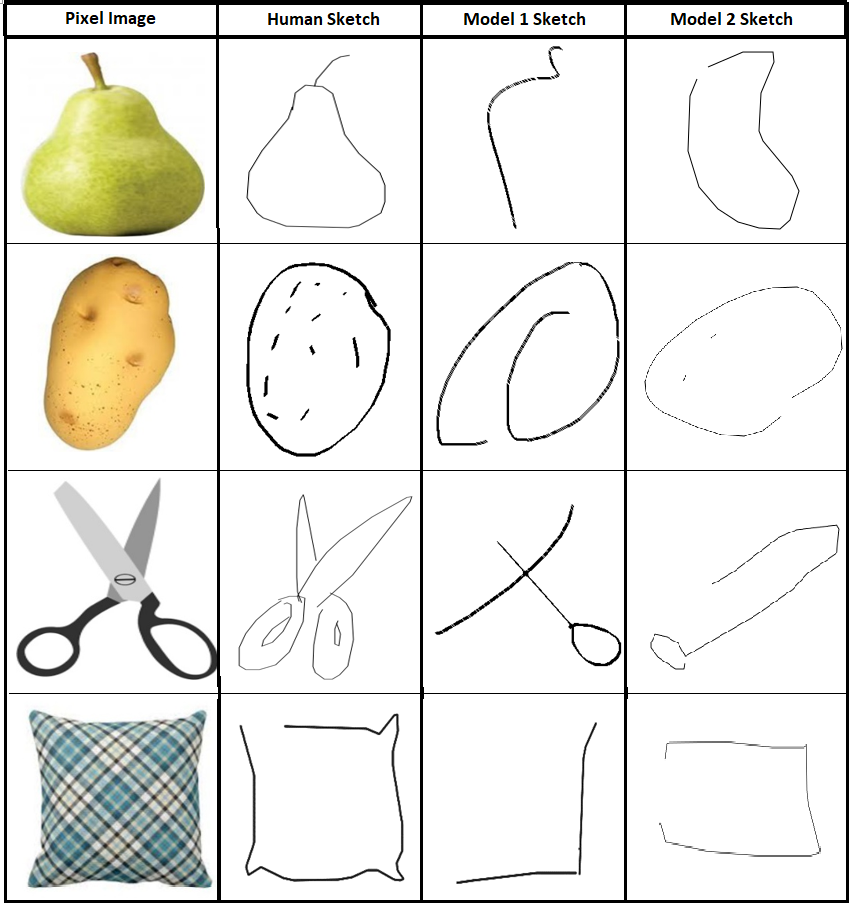
\includegraphics[width=10cm]{images/image.png}
\caption{The leftmost images in each row are the pixel images, the second one is a human drawn sketch, third column of images were generated by LSTM RNN Model and the last column by the LSTM Sketch RNN Model}
\label{fig:sketches}
\end{figure}




\begin{comment}
\begin{figure}[H]
\centering
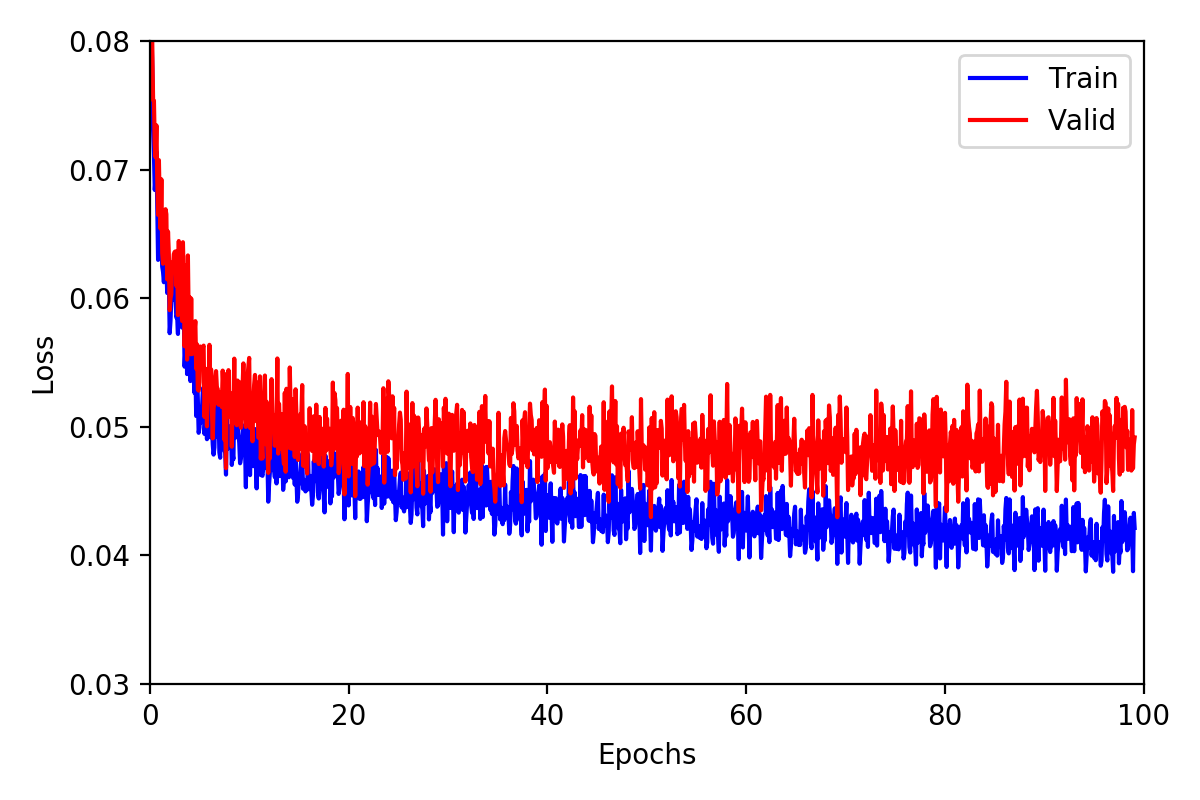
\includegraphics[width=6cm]{images/lossplot.png}
\caption{Training and Validation Loss vs Epoch}
\label{fig:loss}
\end{figure}
\end{comment}
\section{Discussion and Analysis}

\subsection{Quantitative}

As seen in table \ref{table:results_model1}, the quantitative measures indicate quite poor performance of the model on an aggregate. The number of the strokes between the model-drawn sketches and human-sketches are largely uncorrelated, for both CNN-RNN and CNN-Sketch-RNN. This is because the distribution of the pen-down indicator is very skewed, and hence, it is very hard for the model to learn the stroke dynamics. The normalized DTW scores indicate that human-drawn strokes are much more similar to the reference strokes compared to the ones from the model. This poor performance can be attributed to many factors, as detailed in the qualitative analysis, such as inadequate training data for the images and lack of lower level CNN features for edge-detection in the images.

\subsection{Qualitative}

Some sketches generated by the model have been shown in Figure \ref{fig:sketches}. In some cases, the predicted sketch is able to capture the general shape of the object in the pixel image e.g. pixel images of circular objects like the potato in Figure \ref{fig:sketches} are sketched out as a circle. Though some images are seen to be incomplete like the sketch only drew the object halfway or some components of the objects are missing from the sketch e.g. in Figure \ref{fig:sketches}, the pillow is only 2 edges of the 4 edges total and the pair of scissors is missing the handle.

It can be seen the quality of generated sketches is very poor. Also compared to the human sketches, the details that distinguish the objects from general shapes are also lost. In fact, some predicted sketches put the pen down on the first step which means that the sketches are blank. The main reason for this is that the model has a high bias for predicting $p_{1} = 1$ and thus once the pen is put down, it is never lifted up and so there is almost always a single stroke in each sketch. However, the model does seem to recognize some patterns as it can be seen that it draws a round shape for potato and a crossed shape for scissors.

\section{Conclusion}

In this paper, we have described our formulation of the problem of generation of vector images from pixel images. For the data collection, have also proposed a clustering-based technique to form image-sketch pairs that we use to train and evaluate the model. As an initial approach, we have discussed our implementation of a CNN- RNN model and brought about slight improvements using GMMs. Lastly, we have also formulated different quantitative evaluation metrics for the generated sketch images to compare the different models against human-generated sketches. 

As future work, we propose using more refined features of the sketches (pre-trained VGG-net/sketch-RNN features) to form better clusters and have a variable number of clusters per category determined by heuristics over the clustering loss. The lower layers extract lower level features like edges which we want to be drawn by the sketches. Some future work could also be training in phases where we train the LSTM by holding the CNN with the VGG weights in the first phase then fine-tune the weights of the CNN in the second phase. We also propose collecting more pixel images depending on the complexity and requirement of our final model.

Another potential future work could be to change the model to a VAE which restricts the latent variable $z$ i.e. the output of the encoder to be from a unit Gaussian distribution\cite{journals/corr/KingmaW13}. This allows for easier image generation because we know how to sample from a unit Gaussian and that can be used to generate the sketches, unlike the current implementation where we do not know the distribution of the latent variable. With the problem being relatively new, we believe that there are many more interesting insights that can be drawn from the data and performance of the different models, and the models we present could serve as a good starting point for further explorations.

{
\bibliographystyle{unsrtnat}
\bibliography{egbib}
}

\end{document}